\documentclass[../main/main.tex]{subfiles}

\newdate{date}{04}{11}{2020}


\begin{document}

\marginpar{ \textbf{Laboratory 12.} \\  \displaydate{date}. \\ Compiled:  \today.}

\section{Collegare termometro Pt100}

Lo schema del termometro Pt100 è come mostrato in Fig. \ref{fig:12_1}.

\begin{figure}[h!]
\centering
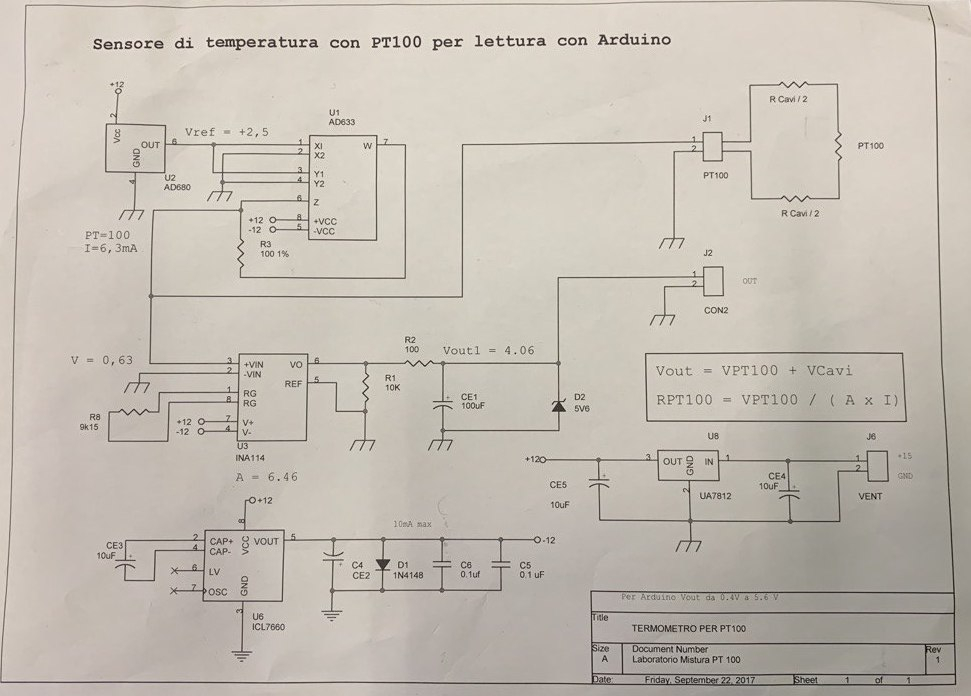
\includegraphics[width=1\textwidth]{../lessons/image/12/1.jpg}
\caption{\label{fig:12_1} Schema termometro Pt100.}
\end{figure}

\marginpar{
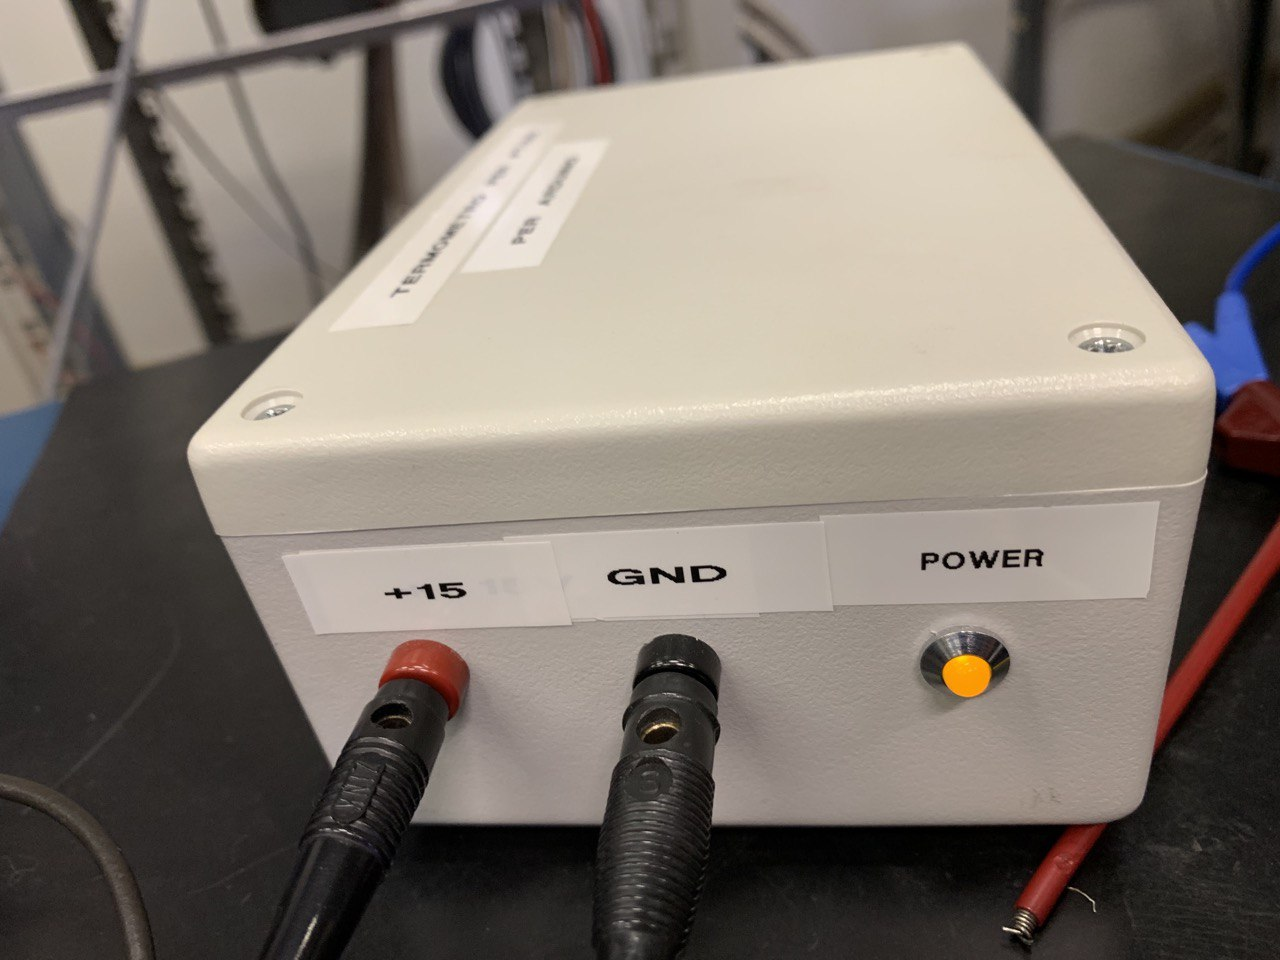
\includegraphics[width=\marginparwidth]{../lessons/image/12/2.jpg}
\captionof{figure}{\label{fig:12_2} Alimentazione termometro.}
}
Abbiamo alimentato il termometro Pt100 con +15 V e collegamento a terra, vedi Fig. \ref{fig:12_2}.
Dopodichè, questo deve essere collegato alla camera a vuoto del criostato. Ci sono quattro collegamenti nel retro.
Se si misura la resistenza tra i due banana più alti o tra i due banana più bassi si misura:
\begin{equation*}
  R_{\text{alto}} = 6.5 \, \Omega, \qquad  R_{\text{basso}} = 7.1 \, \Omega
\end{equation*}
Questa è la resistenza dei cavi resistivi collegati al termometro all'interno della camera (sono cavi speciali perchè non portano fuori il calore). Bisogna tener conto della media di queste resistenze per inserire il suo valore nel programma di LabView e sottrarlo al valore di tensione ottenuto (quindi bisogna effettuare una correzione).

Invece, misurando la resistenza tra le due banane di sinistra o le due banane di destra (dove destra e sinistra si riferiscono al guardando da dietro il criostato, cioè come se l'operatore è dietro e guardasse le banana), si ottiene:
\begin{equation*}
  R_{Pt100}^{\text{sinistra}} = 114.9 \, \Omega,  \qquad R_{Pt100}^{\text{destra}} = 114.5 \, \Omega
\end{equation*}

Abbiamo testato prima il funzionamento del terometro con una resistenza da circa 100 \( \Omega  \) (con più esattezza 98.5 \( \Omega  \)). La colleghiamo ai capi degli ingressi del termometro. Misuriamo 4 V. Il supporto per arduino del terometro funziona, quindi siamo pronti a collegarlo al termometro vero e proprio.

\section{Come funziona il criostato}

Bisogna aprire la pompa da vuoto della camera. Aspettare che la pressione arrivi a circa \( 10^{-3} \) o \( 10^{-2} \). Aprire l'acqua per il raffreddamento ed accendere il criocooler.
Vediamo che la temperatura inizia a scendere. Per arrivare a circa 70 K, il sistema ha impiegato circa 2 ore. L'andamento del raffreddamento è circa lineare.

\begin{remark}
C'è il compressore, circolo termodinamico  che raffredda. E' alimentato ad acqua. Vedere la temperatura dell'acqua per capire se alimentare ancora o no (se è troppo calda continuare ad alimentare).
\end{remark}

Accendere il lock-in e calibrare.
Infatti, già raggiungendo i 273 K dovremmo riuscire a bilanciare il ponte. Però non siamo riuscite.

\section{Errori trovati nel circuito del ponte (termometro)}


In questa lezione abbiamo poi risolto problemi che abbiamo riscontrato nella saldatura del circuito precedente: il circuito del termometro aveva almeno tre errori:
\begin{itemize}
\item avevamo cortocircuitato le due resistenze \( R_1 \) e \( R_2 \);
\item un filo verde che collegava \( V_g \) non era stato collegato (errore banale di connessione ma che poteva costarci tanto);
\item errore più grave di tutti: misuravamo il segnale tra \( R_1 \) e la terra. Invece dobbiamo misurare il segnale tra \( R_1 \) e \( R_2 \)!
\end{itemize}
Abbiamo sistemato tutti questi errori e abbiamo testato il circuito con una resistenza da circa 100 \( \Omega  \). Quest'ultimo funziona in questo caso, mentre non siamo in ogni caso riusciti a bilanciare il ponte collegato la nostra resistenza del termometro.

Il circuito finale è come in Fig. \ref{fig:12_3} e Fig. \ref{fig:12_4}. Notiamo che rispetto alle altre versioni abbiamo anche invertito le boccole 7 e 8 (le altre volte sbagliavamo). Infatti, il capo cortocircuitato è 8 che deve essere connesso alla resistenza $R_1$.

\begin{figure}[h!]
\centering
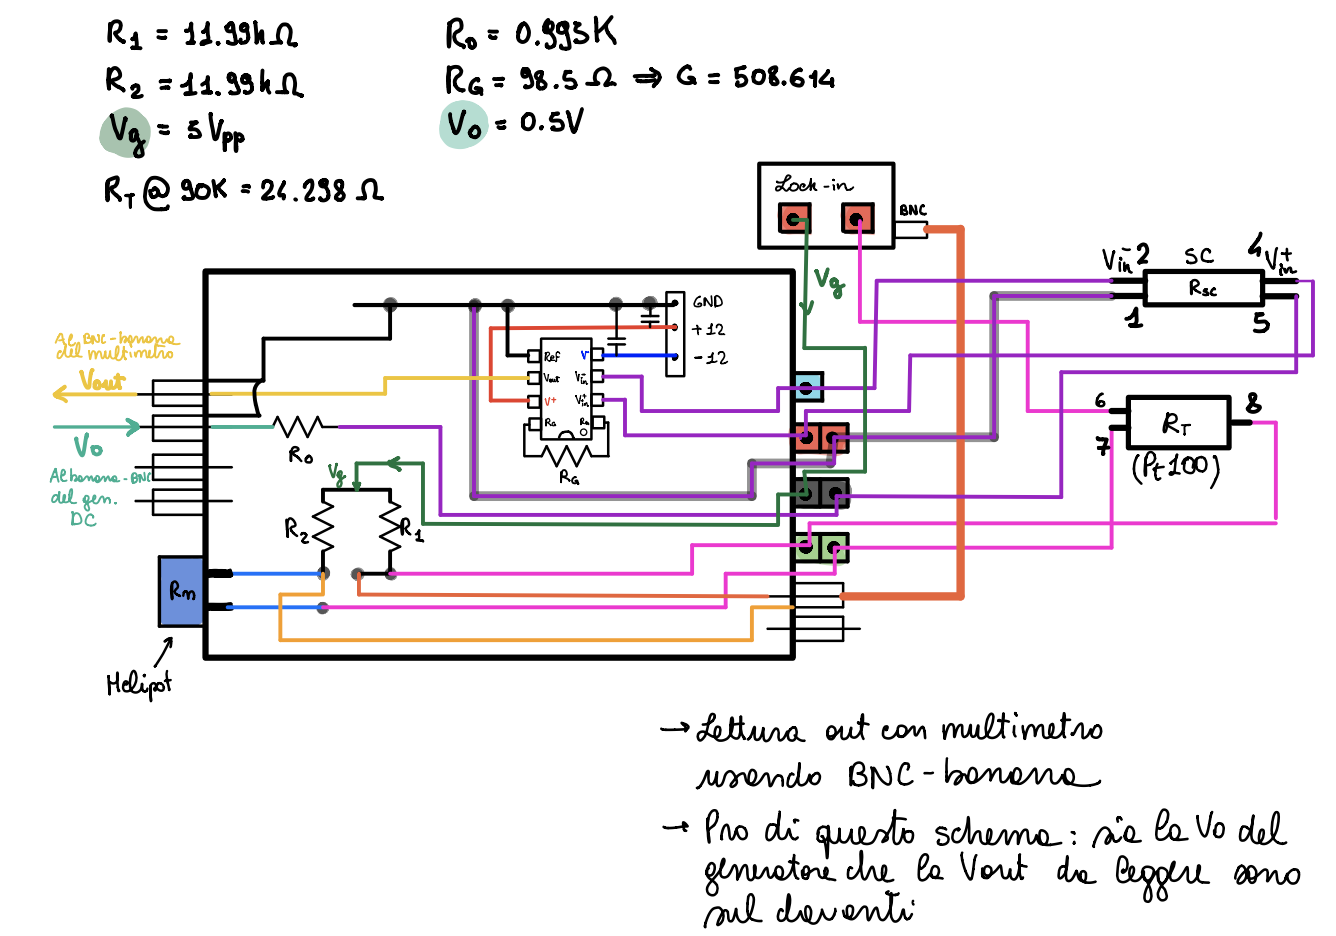
\includegraphics[width=0.8\textwidth]{../lessons/image/12/3.png}
\caption{\label{fig:12_3} Schema circuito finale.}
\end{figure}

\begin{figure}[h!]
\centering
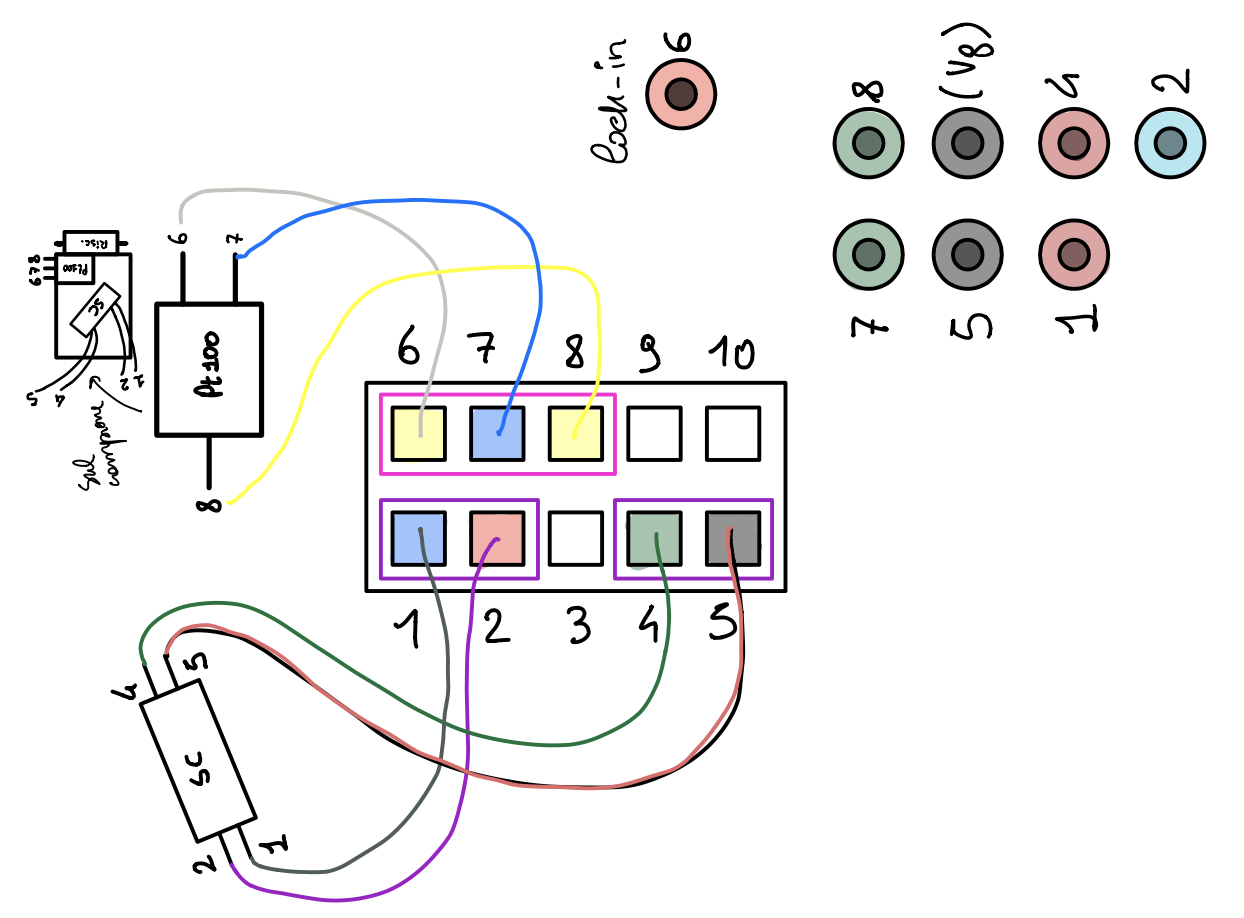
\includegraphics[width=0.8\textwidth]{../lessons/image/12/4.png}
\caption{\label{fig:12_4} Schema boccole finale.}
\end{figure}


\end{document}
